%%%%%%%%%%%%%%%%%%%%%%%%%% AULA 04 %%%%%%%%%%%%%%%%%%%%%%%%%%

%%%%%%%%%%%%%%%%%%%%%%% FINALIDADE %%%%%%%%%%%%%%%%%%%%%%%%%%
%			Demonstrar comandos sobre macros e				%
%			comandos especiais								%
%%%%%%%%%%%%%%%%%%%%%%% FIM FINALIDADE %%%%%%%%%%%%%%%%%%%%%%

%%%%%%%%%%% SLIDE 01 %%%%%%%%%%%%%%%%%%%%%%%%
\begin{frame}{Produzindo verbatim}
	Use o ambiente \Lenv{verbatim} ou o comando \LCmd{verb}. O argumento de \LCmd{verb} deve ser delimitado por dois caracteres como \texttt{+} ou \texttt{=},~\textbf{escolha do usuário}; o caracter não deve ser presente na(s) palavra(s) a ser(em) reproduzida(s) verbatim (literalmente). 
	
	\pause

	\begin{Codigo}{Modo verbatim}
		\LCmd{verb}=\bs LaTeX= \n
		ou\n
		\LCmdArg{begin}{verbatim}\n
			\bs LaTeX\n
		\LCmdArg{end}{verbatim}
	\end{Codigo}

    \pause
	Produz:

	\begin{Resultado}{}
		\texttt{\bs LaTeX}
	\end{Resultado}

    \pause
	\begin{Observacao}{Observação}
		Reproduz o comando sem interpretá-lo.
	\end{Observacao}
\end{frame}
%%%%%%%%%%% FIM SLIDE 01 %%%%%%%%%%%%%%%%%%%%

%%%%%%%%%%% SLIDE 02 %%%%%%%%%%%%%%%%%%%%%%%%
\begin{frame}[fragile]
\frametitle{Usando verbatim para compor programas}

	\begin{Resultado}{Exemplo de resultado}
		{\scriptsize
		\begin{verbatim}
			int f91 (int n){
			  if (n <= 100){
			    return f91 (f91 (n + 11));
			  }else{ 
			    return (n - 10);
			  }
			}
		\end{verbatim}
		}
	\end{Resultado}
\end{frame}
%%%%%%%%%%% FIM SLIDE 02 %%%%%%%%%%%%%%%%%%%%

%%%%%%%%%%% SLIDE 03 %%%%%%%%%%%%%%%%%%%%%%%%
\begin{frame}{Contadores - 0}
	Contadores são uma parte essencial do \LaTeX . Representando o mecanismo principal para numeração de todos os elementos (Listas, legendas, capítulos,...). Para criar um contador novo basta usar o comando:

    \pause
	\begin{Codigo}{}
		\LCmdArg{newcounter}{nome-do-contador}
	\end{Codigo}

    \pause
	Ou ainda pode-se relacionar contadores de maneira que um contador seja zerado toda vez que um outro for incrementado.
	
	\pause
	\begin{Codigo}{}
		\LCmdArg{newcounter}{nome-do-contador}\Larg{outro-contador}
	\end{Codigo}
\end{frame}
%%%%%%%%%%% FIM SLIDE 03 %%%%%%%%%%%%%%%%%%%%

%%%%%%%%%%% SLIDE 04 %%%%%%%%%%%%%%%%%%%%%%%%
\begin{frame}{Contadores - 1}
	\begin{center}
		\begin{tabular}{lp{4cm}}
			\LCmdArg{stepcounter}{NomeContador}& Incrementa um\\
			\pause
			\LCmdArg{refstepcounter}{NomeContador}& Incrementa um e mostra o valor \\
			\pause
			\LCmdArg{addtocounter}{NomeContador}\Larg{num}& Incrementa valor em $num$ \\
			\pause
			\LCmdArg{setcounter}{NomeContador}\Larg{num}& Mudar o valor para $num$ \\
		\end{tabular}
	\end{center}
\end{frame}
%%%%%%%%%%% FIM SLIDE 04 %%%%%%%%%%%%%%%%%%%%

%%%%%%%%%%% SLIDE 05 %%%%%%%%%%%%%%%%%%%%%%%%
\begin{frame}{Contadores - 2}
	\begin{center}
		\begin{tabular}{ll}
			Comando & Exemplo\\
			\hline
			\LCmd{arabic}  & 1,2,3\\
			\LCmd{alph}  & a,b,c\\
			\LCmd{Alph}  & A,B,C\\
			\LCmd{roman}  & i,ii,iii\\
			\LCmd{Roman}  & I,II,III\\
		\end{tabular}
	\end{center}
\end{frame}
%%%%%%%%%%% FIM SLIDE 05 %%%%%%%%%%%%%%%%%%%%

%%%%%%%%%%% SLIDE 06 %%%%%%%%%%%%%%%%%%%%%%%%
\begin{frame}{Definindo o layout da página}
	\begin{itemize}
		\item \LCmdArg{setlength}{parâmetro}\Larg{valor};
		\pause
		\item[] Exemplos de parâmetros:
			\begin{itemize}
				\item \LCmd{parindent} -- endentação do parágrafo;
				\pause
				%\item \LCmd{hoffset} e \LCmd{voffset} -- margens laterais esquerda e superior (mais uma polegada!);
				\item \LCmd{oddsidemargin} -- distância entre margem esquerda lateral e texto na página ímpar (mais uma polegada!);
				\pause
				\item \LCmd{evensidemargin}  -- distância entre margem esquerda lateral e texto na página par (mais uma polegada!);
				\pause
				\item \LCmd{textwidth} e \LCmd{textheight} -- tamanho da área de texto.
			\end{itemize}
	\end{itemize}

    \pause
	\begin{Observacao}{Observação}
		Na atual versão de \LaTeX{} é melhor tratar o layout da página usando o pacote \Lsty{geometry}.
	\end{Observacao}
\end{frame}
%%%%%%%%%%% FIM SLIDE 06 %%%%%%%%%%%%%%%%%%%%

%%%%%%%%%%% SLIDE 07 %%%%%%%%%%%%%%%%%%%%%%%%
\begin{frame}[fragile]
\frametitle{Pacote \texttt{geometry}}\fontsize{10}{11}\selectfont

	Exemplos de uso:
	
	\begin{itemize}
		\item \verb+\usepackage[text={17.8cm,25.4cm},centering]{geometry}+ -- layout de página com texto de 17,8 cm de largura e 25,4 cm de altura centralizado;
		\pause
		\item \verb+\usepackage[total={16.5cm,22.2cm},top=3cm,+ \verb+left=2.3cm, includefoot]{geometry}+ -- texto de 16,5 cm de largura, 22,2 cm de altura, margem superior de 3 cm e lateral esquerdo de 2,3 cm, com número de página no rodapé.
	\end{itemize}
\end{frame}
%%%%%%%%%%% FIM SLIDE 07 %%%%%%%%%%%%%%%%%%%%

%%%%%%%%%%% SLIDE 08 %%%%%%%%%%%%%%%%%%%%%%%%
\begin{frame}{Unidades usadas pelo \TeX}
	\begin{Codigo}{Algumas unidades usadas pelo \TeX}
		\begin{tabular}{ll}
			\texttt{pt} & pontos \\
			\texttt{mm} & milímetros \\
			\texttt{cm} & centímetros \\
			\texttt{in} & polegadas \\
			\texttt{ex} & altura da letra ``x'' no fonte corrente \\
			\texttt{em} & largura da letra ``m'' no fonte corrente
		\end{tabular}
	\end{Codigo}
\end{frame}
%%%%%%%%%%% FIM SLIDE 08 %%%%%%%%%%%%%%%%%%%%

%%%%%%%%%%% SLIDE 09 %%%%%%%%%%%%%%%%%%%%%%%%
\begin{frame}{Ambiente \Lenv{thebibliography} - 0}
	\begin{Codigo}{Exemplo de bibliografia}
		\LCmdArg{begin}{thebibliography}\Larg{1}\n
			\LCmdArg{bibitem}{bib:lamport} Lamport, Leslie\n
			\LCmdArg{emph}{\LCmd{LaTeX}: A Document Preparation System}, Addison-Wesley Publishing Company, 2nd edition,1994.
			\LCmdArg{bibitem}{bib:goossens} Goossens, Michel and\n 
			 Mittelbach, Frank and Samarin, Alexander\n
			\LCmdArg{emph}{The \LCmd{LaTeX}\LCmd{ }Companion},\n 
			Addison-Wesley, 1994.\n
		\LCmdArg{end}{thebibliography}
	\end{Codigo}
\end{frame}
%%%%%%%%%%% FIM SLIDE 09 %%%%%%%%%%%%%%%%%%%%

%%%%%%%%%%% SLIDE 10 %%%%%%%%%%%%%%%%%%%%%%%%
\begin{frame}{Ambiente \Lenv{thebibliography} - 1}
	\begin{Resultado}{Exemplo de bibliografia}
		\begin{thebibliography}{1}
			\bibitem{bib:lamport} Lamport, Leslie
				\emph{\LaTeX: A Document Preparation System},
				Addison-Wesley Publishing Company, 2nd edition, 1994.
			\bibitem{bib:goossens} Goossens, Michel and
				Mittelbach, Frank and Samarin, Alexander
				\emph{The \LaTeX\ Companion},
				Addison-Wesley, 1994.
		\end{thebibliography}
	\end{Resultado}
\end{frame}
%%%%%%%%%%% FIM SLIDE 10 %%%%%%%%%%%%%%%%%%%%

%%%%%%%%%%% SLIDE 11 %%%%%%%%%%%%%%%%%%%%%%%%
\begin{frame}{Citações}
	Para citar, use o comando \LCmdArg{cite}{\dots}.

	\begin{Codigo}{Exemplo}
		O livro de Leslie Lamport \LCmdArg{cite}{bib:lamport} é o clássico de \LCmd{LaTeX}.
	\end{Codigo}

    \pause
	Produz:

	\begin{Resultado}{}
		O livro de Leslie Lamport \cite{bib:lamport} é o clássico de \LaTeX.
	\end{Resultado}
\end{frame}
%%%%%%%%%%% FIM SLIDE 11 %%%%%%%%%%%%%%%%%%%%

%%%%%%%%%%% SLIDE 12 %%%%%%%%%%%%%%%%%%%%%%%%
\begin{frame}{Usando BiB\TeX - 0}
	\begin{itemize}
		\item BiB\TeX\ é um programa externo que permite definir referências bibliográficas;
		\pause
		\item Usa um banco de dados definido em um arquivo .BIB;
		\pause
		\item São importadas apenas as referências indicadas nos comandos \LCmd{cite} e \LCmd{nocite};
		\pause
		\item O programa \prog{bibtex} lê o arquivo .AUX gerado pelo \LaTeX;
	\end{itemize}
\end{frame}
%%%%%%%%%%% FIM SLIDE 12 %%%%%%%%%%%%%%%%%%%%

%%%%%%%%%%% SLIDE 13 %%%%%%%%%%%%%%%%%%%%%%%%
\begin{frame}{Usando BiB\TeX - 1}
	\begin{itemize}
		\item O comando \LCmdArg{bibliography}{nome} informa que a bibliografia encontra-se no arquivo \texttt{nome.bib};
		\pause
		\item O comando \LCmdArg{bibliographystyle}{estilo} define o estilo da bibliografia a ser produzida (estilos disponíveis: \Lsty{plain}, \Lsty{unsrt} e \Lsty{alpha} e muitos outros).
	\end{itemize}
\end{frame}
%%%%%%%%%%% FIM SLIDE 13 %%%%%%%%%%%%%%%%%%%%

%%%%%%%%%%% SLIDE 14 %%%%%%%%%%%%%%%%%%%%%%%%
\begin{frame}{Criação e uso do banco de dados bibliográfico}
	Passos para obter as referências bibliográficas:

	\begin{enumerate}
		\item Edite o arquivo .BIB com as referências (por exemplo, \texttt{teste.bib});
		\pause
		\item Edite o arquivo .TEX com os comandos \LCmd{cite} e \LCmd{nocite} (por exemplo, \texttt{teste.tex});
		\pause
		\item Compile o arquivo .TEX (por exemplo, \texttt{\$ pdflatex teste}), gerando assim o arquivo .AUX que será lido pelo programa \prog{bibtex};
		\pause
		\item Execute o programa \prog{bibtex} (por exemplo, \texttt{\$ bibtex teste});
		\pause
		\item Execute novamente o comando \texttt{pdflatex} para gerar o .PDF com a bibliografia.
	\end{enumerate}
\end{frame}
%%%%%%%%%%% FIM SLIDE 14 %%%%%%%%%%%%%%%%%%%%

%%%%%%%%%%% SLIDE 15 %%%%%%%%%%%%%%%%%%%%%%%%
\begin{frame}{Estrutura do arquivo .BIB}
	Estrutura do arquivo .BIB: Sequência de entradas. Cada entrada é definida como:

    \pause
	\begin{Codigo}{}
		@tipo\Larg{rótulo, chave=valor, chave=valor, \dots}
	\end{Codigo}

    \pause
	\begin{Observacao}{Tipos de entradas mais comuns}
		{\setbeamersize{description width=8em}%
		\begin{description}
			\item [book] livro;
			\item [inproceedings] artigo em anais de evento;
			\item [article] artigo em periódico.
		\end{description}}
	\end{Observacao}
\end{frame}
%%%%%%%%%%% FIM SLIDE 15 %%%%%%%%%%%%%%%%%%%%

%%%%%%%%%%% SLIDE 16 %%%%%%%%%%%%%%%%%%%%%%%%
\begin{frame}{Banco de dados .BIB}
\fontsize{9}{10}\selectfont

	\begin{Codigo}{Exemplo}
		@inproceedings\{bib:campani,\n
			author = \string"Carlos A. P. Campani and Paulo Blauth Menezes\string",\n
			title = \string"Characterizing the Software Development Process: A New Approach Based on \{K\}olmogorov Complexity\string",\n
			booktitle = \string"\{Computer Aided Systems Theory - EUROCAST'2001, 8th International Workshop on Computer Aided Systems Theory\}\string",\n
			pages = \string"242-256\string",\n
			year = \string"2001\string",\n
			editor = \string"\{Moreno-Díaz and Buchberger and Freire\}\string",\n
			volume = 2178,\n
			series = \string"\{Lecture Notes in Computer Science\}\string",\n
			publisher = \string"Springer\string" \}
		\nn
		@book\{bib:li,\n
			author = \string"Ming Li and Paul Vit\string\'\{a\}nyi\string",\n
			title = \string"An Introduction to \{K\}olmogorov Complexity and its Applications\string",\n
			publisher = \string"Springer\string",\n
			address = \string"\{New York\}\string",\n
			year = 1997 \}
	\end{Codigo} 
\end{frame}
%%%%%%%%%%% FIM SLIDE 16 %%%%%%%%%%%%%%%%%%%%

%%%%%%%%%%% SLIDE 17 %%%%%%%%%%%%%%%%%%%%%%%%
\begin{frame}{Produzindo o index}
	\begin{itemize}
		\item Usar o programa externo \prog{makeindex};
		\pause
		\item Importar pacote \Lsty{makeidx};
		\pause
		\item Habilitar com o comando \LCmd{makeindex};
		\pause
		\item Cada entrada do index é especificada no texto usando o comando \LCmdArg{index}{chave};
		\pause
		\item \LaTeX\ produz um arquivo .IDX.
	\end{itemize}
\end{frame}
%%%%%%%%%%% FIM SLIDE 17 %%%%%%%%%%%%%%%%%%%%

%%%%%%%%%%% SLIDE 18 %%%%%%%%%%%%%%%%%%%%%%%%
\begin{frame}{Alguns exemplos de sintaxe das chaves}
	\begin{flushleft}
		\begin{tabular}{ll}
			\toprule
			\multicolumn1c{No arquivo .TEX}     &\multicolumn1c{No texto composto}\\
			\midrule
			\LCmdArg{index}{complexidade}           & complexidade, 10 \\
			\LCmdArg{index}{Alcorão Sagrado} & Alcorão Sagrado, 99 \\
			\LCmdArg{index}{complexidade!definição}& complexidade \\
                    & \hspace{6mm}definição, 22 \\
			\LCmdArg{index}{Kolmogorov|textbf}  & Kolmogorov, \textbf{31}\\
			\bottomrule
		\end{tabular}
	\end{flushleft}

	\medskip

    \pause
	\begin{Observacao}{Observação}
		O index é produzido no lugar em que ocorrer o comando \LCmd{printindex}.
	\end{Observacao}
\end{frame}
%%%%%%%%%%% FIM SLIDE 18 %%%%%%%%%%%%%%%%%%%%

%%%%%%%%%%% SLIDE 19 %%%%%%%%%%%%%%%%%%%%%%%%
\begin{frame}{Criar o index}
	\begin{Codigo}{Exemplo}
		\LCmdArg{documentclass}{book}\n
		\dots\n
		\LCmdArg{usepackage}{makeidx}\n
		\LCmd{makeindex}\n
		\LCmdArg{begin}{document}\n
			A complexidade\LCmdArg{index}{complexidade} de Kolmogorov \dots\n
			\LCmd{printindex}\n
		\LCmdArg{end}{document}
	\end{Codigo}

    \pause
	Para processar o arquivo .IDX:
	
	\begin{Codigo}{}
		\$ pdflatex teste \n
		\$ makeindex teste \n
		\$ pdflatex teste \n
	\end{Codigo}
\end{frame}
%%%%%%%%%%% FIM SLIDE 19 %%%%%%%%%%%%%%%%%%%%

%%%%%%%%%%% SLIDE 20 %%%%%%%%%%%%%%%%%%%%%%%%
\begin{frame}{Ambiente \Lenv{picture}}
	\begin{itemize}
		\item Permite desenhar figuras vetoriais.

            \pause
			\begin{Codigo}{Sintaxe}
				\LCmdArg{begin}{picture}(largura,altura)(x-orig,y-orig)\n
					comandos de \Lsty{picture} \dots\n
				\LCmdArg{end}{picture}
			\end{Codigo}

        \pause
		\item As limitações do ambiente \Lenv{picture} podem ser superadas pelo uso do pacote \Lsty{pict2e}.
	\end{itemize}
\end{frame}
%%%%%%%%%%% FIM SLIDE 20 %%%%%%%%%%%%%%%%%%%%

%%%%%%%%%%% SLIDE 21 %%%%%%%%%%%%%%%%%%%%%%%%
\begin{frame}{Uso de \Lenv{picture} - 0}
	\begin{Codigo}{Exemplo}
		\LCmdArg{begin}{picture}(60,30)(0,15)\n
			\LCmd{Line}(0,0)(15,0) \n
			\LCmd{polygon}(15,-9)(15,9)(33,0)  \n
			\LCmd{put}(36,0)\Larg{\LCmd{circle}\Larg{6}} \n
			\LCmd{Line}(39,0)(54,0) \n
		\LCmdArg{end}{picture}
	\end{Codigo}

    \pause
	Produz:

	\begin{Resultado}{}\centering
		\begin{picture}(60,30)(0,-15)
			\Line(0,0)(15,0) 
			\polygon(15,-9)(15,9)(33,0) 
			\put(36,0){\circle{6}}
			\Line(39,0)(54,0)
		\end{picture}
	\end{Resultado}
\end{frame}
%%%%%%%%%%% FIM SLIDE 21 %%%%%%%%%%%%%%%%%%%%

%%%%%%%%%%% SLIDE 22 %%%%%%%%%%%%%%%%%%%%%%%%
\begin{frame}{Uso de \Lenv{picture} - 1}
	\begin{Codigo}{Outro exemplo}
		\LCmdArg{begin}{picture}(65,30)(0,15)\n
			\LCmd{put}(0,0)\Larg{\LCmd{arc}\LOpt{45,-45}\Larg{22}}\n
			\LCmd{Line}(0,7)(21,7)\LCmd{Line}(0,-7)(21,-7)\n
			\LCmd{put}(15.56,-35)\Larg{\LCmd{arc}\LOpt{90,45}{50.5}}\n
			\LCmd{put}(15.56,+35)\Larg{\LCmd{arc}\LOpt{-90,-45}{50.5}}\n
			\LCmd{put}(52,0)\Larg{\LCmd{circle}{2.5}}\LCmd{Line}(54,0)(65,0)\n
		\LCmdArg{end}{picture}
	\end{Codigo}

    \pause
	Produz:

	\begin{Resultado}{}\centering
		\begin{picture}(65,30)(0,-15)
			\put(0,0){\arc[45,-45]{22}}
			\Line(0,7.)(21,7)\Line(0,-7)(21,-7)
			\put(15.56,-35){\arc[90,45]{50.5}}
			\put(15.56,+35){\arc[-90,-45]{50.5}}
			\put(52,0){\circle{2.5}}
			\Line(53,0)(65,0)
		\end{picture}
	\end{Resultado}
\end{frame}
%%%%%%%%%%% FIM SLIDE 22 %%%%%%%%%%%%%%%%%%%%

%%%%%%%%%%% SLIDE 23 %%%%%%%%%%%%%%%%%%%%%%%%
\begin{frame}{O pacote \Xy-pic}
	\begin{itemize}
		\item Usado para desenhar diagramas, autômatos, teoria das categorias, etc;
		\pause
		\item Fornece uma notação mnemônica e consistente, baseada na composição lógica de componentes visuais;
		\pause
		\item \LOA usepackage[all]{xy};
		\pause
		\item Veja:~\scriptsize{\url{http://www.ufpel.edu.br/~campani/xypictutorial.pdf}}.
	\end{itemize}
\end{frame}
%%%%%%%%%%% FIM SLIDE 23 %%%%%%%%%%%%%%%%%%%%

%%%%%%%%%%% SLIDE 24 %%%%%%%%%%%%%%%%%%%%%%%%
\begin{frame}{Exemplos do pacote \Xy-pic - 0}
	\begin{Codigo}{Primeiro exemplo}
		\LCmdArg{xymatrix}{\n
			1 \LCmd{ar}\LO[dr] \& 2 \LCmd{\bs}\n
			3         \& 4 \n   
		}
	\end{Codigo}

    \pause
	Produz:
	
	\begin{Resultado}{}
		\[\xymatrix{
		1 \ar[dr] & 2 \\
		3         & 4 }\]
	\end{Resultado}
\end{frame}
%%%%%%%%%%% FIM SLIDE 24 %%%%%%%%%%%%%%%%%%%%

%%%%%%%%%%% SLIDE 25 %%%%%%%%%%%%%%%%%%%%%%%%
\begin{frame}{Exemplos do pacote \Xy-pic - 1}
	\begin{Codigo}{Segundo exemplo}
		\LCmdArg{xymatrix}{\n
			1 \LCmd{ar}\LO[dr]\string^\Larg{A}   \LCmd{\bs}\n
			2 \LCmd{ar@}(dl,d)\LO[]  \& *+\LO[F-]\Larg{3}  \n 
		}
	\end{Codigo}

    \pause
	Produz:
	
	\begin{Resultado}{}
		\[\rule[-65pt]{0pt}{0pt}\xymatrix{
		1 \ar[dr]^{A} \\
		2 \ar@(dl,d)[]  & *+[F-]{3} }\]
	\end{Resultado}
\end{frame}
%%%%%%%%%%% FIM SLIDE 25 %%%%%%%%%%%%%%%%%%%%

%%%%%%%%%%% SLIDE 26 %%%%%%%%%%%%%%%%%%%%%%%%
\begin{frame}{Exemplos do pacote \Xy-pic - 2}
	\begin{Codigo}{Curvando uma seta pontilhada}
		\LCmdArg{xymatrix}{\n
		\LCmdArg{textrm}{Início}\n
		\LCmd{ar@}/\string^/@\Larg{.>}\LO[rr]\string^{\LCmdArg{mathrm}{atalho}}\n 
		\& \LCmdArg{mathrm}{Meio} \& \LCmdArg{mathrm}{Fim}\n
		}
	\end{Codigo}

    \pause
	Produz:

	\begin{Resultado}{}
		\[\xymatrix{
		\textrm{Início} \ar@/^/@{.>}[rr]^{\mathrm{atalho}} & \mathrm{Meio} & \mathrm{Fim}}\]
	\end{Resultado}

    \pause
	\begin{Observacao}{Observação}
		Quando é usado o pacote \Lsty{amsmath} o comando \LCmd{textrm} pode ser usado também em modo matemático; o mesmo por outros comandos \LCmd{text\dots}.
	\end{Observacao}
\end{frame}
%%%%%%%%%%% FIM SLIDE 26 %%%%%%%%%%%%%%%%%%%%

%%%%%%%%%%% SLIDE 27 %%%%%%%%%%%%%%%%%%%%%%%%
\begin{frame}{Exemplos do pacote \Xy-pic - 3}
	\begin{Codigo}{Quarto exemplo}
		\LCmdArg{xymatrix}{ \n
			*++\LO[o]\LO[F-]\Larg{1} \LCmd{ar@}(ul,ul)\LO[] \LCmd{ar}\LO[r]\string^\Larg{1}\n
			\LCmd{ar}\LO[d]\string^\Larg{0} \& *++\LO[o]\LO[F=]\Larg{3} \LCmd{\bs}\n
			*++\LO[o]\LO[F-]\Larg{2} \LCmd{ar}\LO[ur]\string_\Larg{1} \LCmd{ar@}(dl,d) \LO[]\string_\Larg{0} 
		}
	\end{Codigo}

    \pause
	Produz:

	\begin{Resultado}{}
		\[\xymatrix{
			*++[o][F-]{1} \ar@(ul,ul)[] \ar[r]^{1}
			\ar[d]^{0} & *++[o][F=]{3} \\
			*++[o][F-]{2} \ar[ur]_{1} \ar@(dl,d)[]_{0}
		}\]
	\end{Resultado}
\end{frame}
%%%%%%%%%%% FIM SLIDE 27 %%%%%%%%%%%%%%%%%%%%

%%%%%%%%%%% SLIDE 28 %%%%%%%%%%%%%%%%%%%%%%%%
\begin{frame}{Exemplos do pacote \Xy-pic - 4}
	\begin{Resultado}{}
		\[\xymatrix@R=18pt{
			& \mathrm{Khether}\ar@{-}[dl]_{\mathrm{B}}\ar@{-}[ddd]^{\mathrm{G}}\ar@{-}[dr]^{\mathrm{A}} \\
			\mathrm{Binah}\ar@{-}[d]_{\mathrm{Ch}}\ar@{-}[ddr]^(.3){\mathrm{Z}}\ar@{-}[rr]|(.4){\mathrm{D}} & & \mathrm{Chokmah}\ar@{-}[d]^{\mathrm{V}}\ar@{-}[ddl]_(.3){\mathrm{H}} \\
			\mathrm{Geburah}\ar@{-}[rr]|(.4){\mathrm{T}}\ar@{-}[dd]_{\mathrm{M}}\ar@{-}[dr]_{\mathrm{L}} & &
			\mathrm{Chesed}\ar@{-}[dd]^{\mathrm{Kh}}\ar@{-}[dl]^{\mathrm{I}} \\
			& \mathrm{Thiphereth}\ar@{-}[dr]^{\mathrm{N}}\ar@{-}[dl]_{\mathrm{Hw}}\ar@{-}[dd]^(.3){\mathrm{S}} \\
			\mathrm{Hod}\ar@{-}[rr]|(.4){\mathrm{P}}\ar@{-}[dr]^{\mathrm{R}}\ar@{-}[ddr]_{\mathrm{Sh}}
			& & \mathrm{Netsach}\ar@{-}[dl]_{\mathrm{Ts}}\ar@{-}[ddl]^{\mathrm{K}} \\
			& \mathrm{Iesod}\ar@{-}[d]_(.3){\mathrm{Th}} \\
			& \mathrm{Malkhuth}
		}\]
	\end{Resultado}
\end{frame}
%%%%%%%%%%% FIM SLIDE 28 %%%%%%%%%%%%%%%%%%%%

%%%%%%%%%%% SLIDE 29 %%%%%%%%%%%%%%%%%%%%%%%%
\begin{frame}{Exemplos do pacote \Xy-pic - 5}
	\begin{Codigo}{Código parcial do último exemplo}
		\LCmdArg{xymatrix@R=18pt}{ \n
			\& \LCmdArg{mathrm}{Khether}\LCmdArg{ar@}{-}\LO[dl]\string_\Larg{\LCmdArg{mathrm}{B}} \n
			\LCmdArg{ar@}{-}\LO[ddd]\string^\Larg{\LCmdArg{mathrm}{G}} \n
			\LCmdArg{ar@}{-}\LO[dr]\string^\Larg{\LCmdArg{mathrm}{A}}  \LCmd{\bs}\n
			\LCmdArg{mathrm}{Binah}\LCmdArg{ar@}{-}\LO[d]\string_\Larg{\LCmdArg{mathrm}{Ch}} \n
			\LCmdArg{ar@}{-}\LO[ddr]\string^(.3)\Larg{\LCmdArg{mathrm}{Z}} \n
			\LCmdArg{ar@}{-}\LO[rr]|(.4)\Larg{\LCmdArg{mathrm}{D}} \& \&  \n
			\dots \n
			\& \LCmdArg{mathrm}{Malkhuth} \n
		}
	\end{Codigo}
\end{frame}
%%%%%%%%%%% FIM SLIDE 29 %%%%%%%%%%%%%%%%%%%%

%%%%%%%%%%% SLIDE 30 %%%%%%%%%%%%%%%%%%%%%%%%
\begin{frame}{Descrevendo partidas de xadrez -- \texttt{skak}}
	\begin{itemize}
		\item Usa uma notação particular para descrever posições de um tabuleiro de xadrez e os movimentos de uma partida;
		\pause
		\item Permite introduzir comentários;
		\pause
		\item Possui comandos para personalizar o desenho do tabuleiro e outras informações;
		\pause
		\item A documentação completa já existe no \TeX\ Live e pode ser lida com o comando \texttt{texdoc skak} na linha de comandos (Terminal).
	\end{itemize}
\end{frame}
%%%%%%%%%%% FIM SLIDE 30 %%%%%%%%%%%%%%%%%%%%

%%%%%%%%%%% SLIDE 31 %%%%%%%%%%%%%%%%%%%%%%%%
\begin{frame}{Exemplo: Abertura Ruy Lopez}
	\begin{columns}
		\begin{column}{.475\textwidth}
			\begin{Codigo}{Fonte}
				\LCmd{newgame}\n 
					\LCmdArg{mainline}{1.e4 e5 2. Nf3 Nc6 3.Bb5}\n 
					\LCmd{showboard}
			\end{Codigo}
		\end{column}

		\hfill
		
        \pause
		\begin{column}{.475\textwidth}
			\begin{Resultado}\centering
				
\includegraphics[width=\hsize]{Imagens/tabuleiro}
			\end{Resultado}
		\end{column}
	\end{columns}
\end{frame}
%%%%%%%%%%% FIM SLIDE 31 %%%%%%%%%%%%%%%%%%%%

%%%%%%%%%%% SLIDE 32 %%%%%%%%%%%%%%%%%%%%%%%%
\begin{frame}{Produzindo partituras musicais com MusiX\TeX}
	\begin{itemize}
		\item MusiX\TeX{} é incluído no \TeX\ Live;
		\pause
		\item Leia a documentação com o comando \texttt{texdoc musixtex} 
		\pause
		\item Usa notação musical para descrever a partitura;
		\pause
		\item \LCmdArg{usepackage}{musixtex} e \LCmdArg{usepackage}{musixcpt}
		\pause
		\item Rosegarden (sequenciador de midi) -- \url{http://www.rosegardenmusic.com/}
	\end{itemize}
\end{frame}
%%%%%%%%%%% FIM SLIDE 32 %%%%%%%%%%%%%%%%%%%%

%%%%%%%%%%% SLIDE 33 %%%%%%%%%%%%%%%%%%%%%%%%
\begin{frame}{Um exemplo de partitura - 0}
\fontsize{11}{12}\selectfont
	\begin{Codigo}{Fonte da partitura}
		\LCmdArg{begin}{music} \string\hsize=100mm \n
			\LCmdArg{generalmeter}{\string\meterfrac24}\% \n 
			\string\parindent 0pt \string\generalsignature{-3} \n 
			\string\startpiece\string\bigaccid \string\NOtes\string\qu\Larg{ce}\string\en\string\bar \n
			\string\NOtes\string\qu\Larg{gh}\string\en\string\bar \string\NOtes\string\qu\Larg{=b}\string\en  \n
			\string\Notes\string\ds\string\cu g\string\en\string\bar \string\NOtes\string\qu\Larg{\string^f=f}\string\en\string\bar \n
			\string\NOtes\string\qu\Larg{=e}\string\itied0e\string\qu\Larg{\string_e}\string\en\string\bar \n
			\string\Notes\string\ttie0\string\Qqbu ed\Larg{\string_d}c\string\en\string\bar \n
			\string\Notes\string\ibu0b\Larg{-2}\string\qb0\Larg{=b}\string\enotes \n
			\string\notes\string\nbbu0\string\qb0\Larg{=a}\string\tqh0N\string\enotes \n
			\string\Notes\string\Dqbu cf\string\en\string\bar \n
			\string\NOtes\LCmdArg{uptext}{\string\it tr}\string\qu e\%\n
			\LCmdArg{uptext}{\string\it tr}\string\qu d\string\en\string\bar \n
			\string\NOtes\string\qu c\string\qp\string\en\string\Endpiece \n
		\LCmdArg{end}{music} \n
	\end{Codigo}
\end{frame}
%%%%%%%%%%% FIM SLIDE 33 %%%%%%%%%%%%%%%%%%%%

%%%%%%%%%%% SLIDE 34 %%%%%%%%%%%%%%%%%%%%%%%%
\begin{frame}{Um exemplo de partitura - 1}
	\begin{Resultado}{}
		\centering
		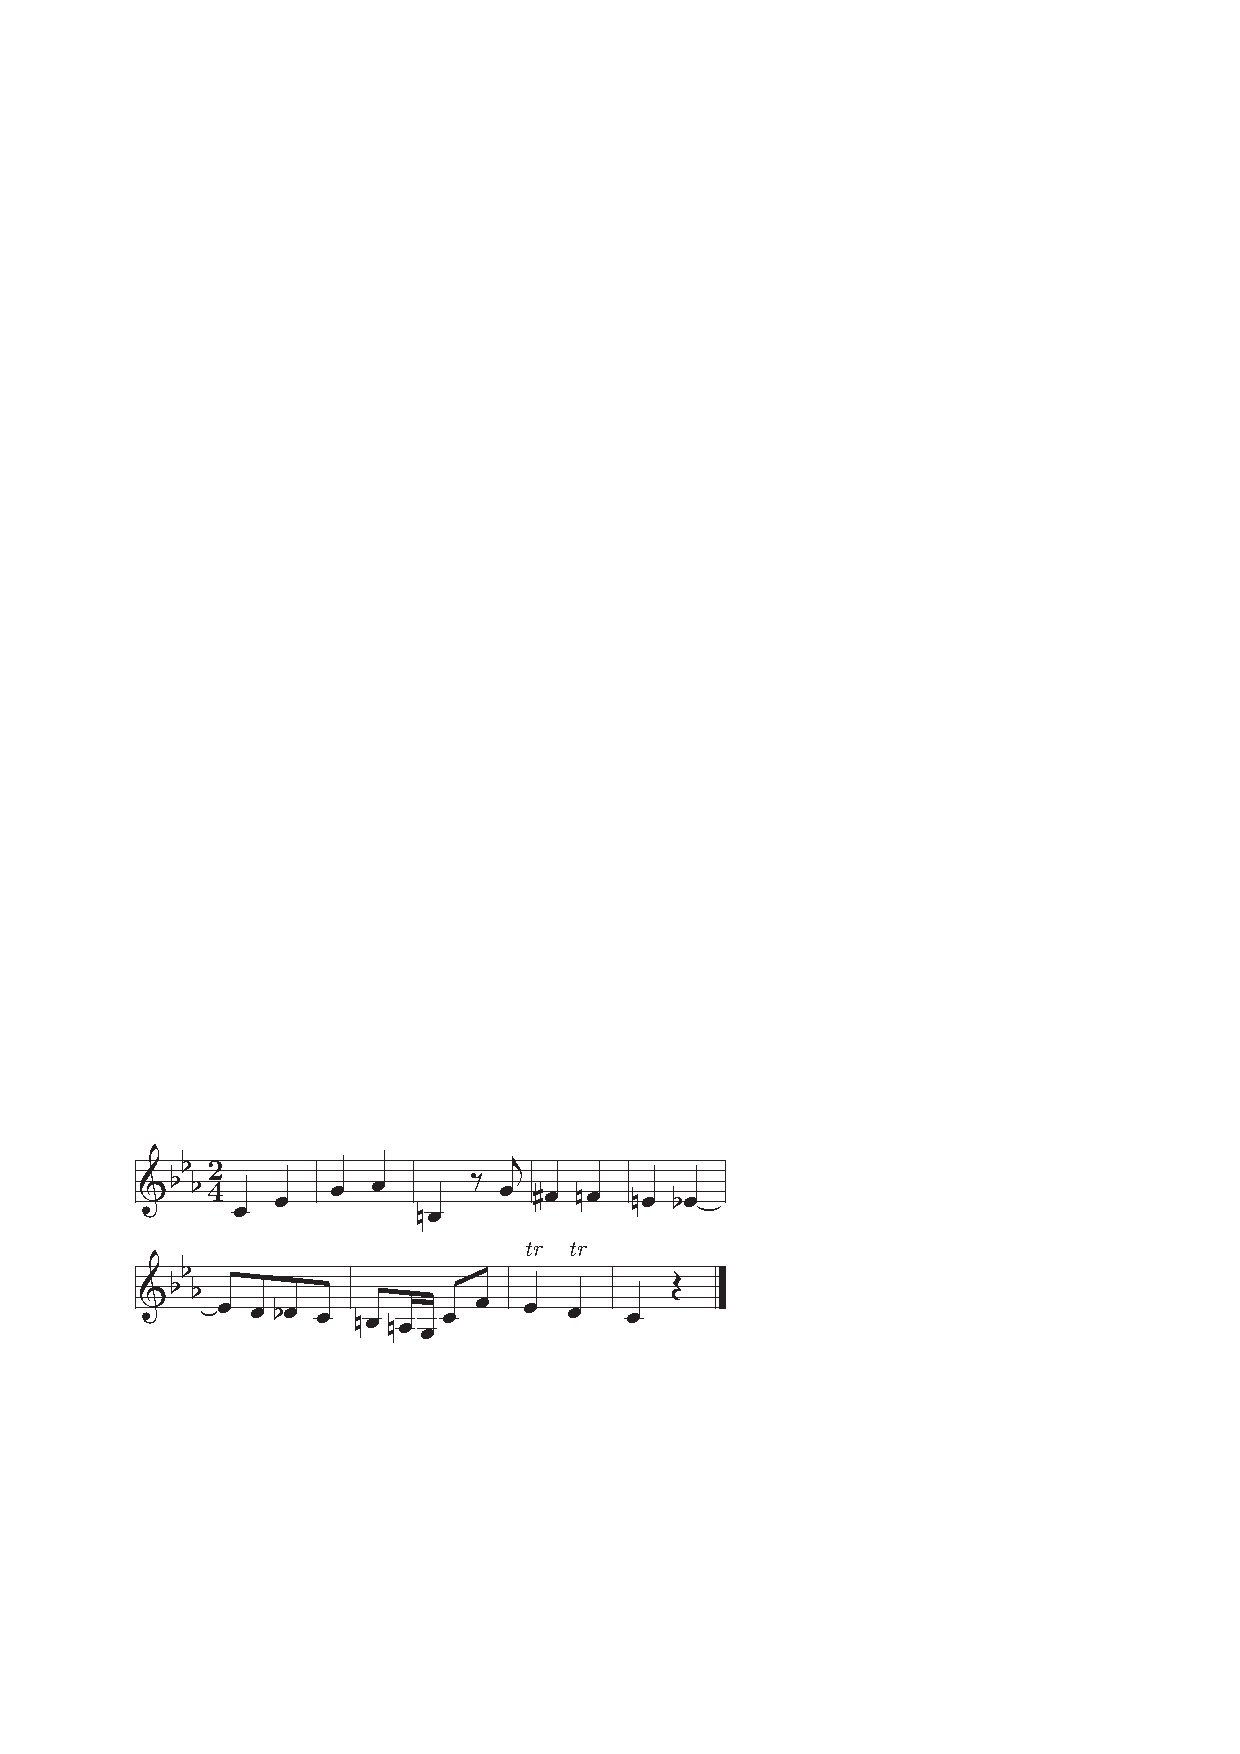
\includegraphics[width=\hsize]{Imagens/Musica}
	\end{Resultado}
\end{frame}
%%%%%%%%%%% FIM SLIDE 34 %%%%%%%%%%%%%%%%%%%%

%%%%%%%%%%% SLIDE 35 %%%%%%%%%%%%%%%%%%%%%%%%
\begin{frame}[fragile]
\frametitle{Fórmulas químicas}
	\begin{itemize}
		\item \LaTeX\ possui pacotes para tipografia de textos científicos que, entre outras coisas, permitem a composição de fórmulas químicas;
		\pause
		\item Evita o excesso de subscritos típicos desse tipo de aplicação;
		\pause
		\item Leia a documentação com o comando \texttt{texdoc mhchem};
		\pause
		\item \LCmdOptArg{usepackage}{version=3}{mhchem}
	\end{itemize}

    \pause
	\begin{Codigo}{Exemplo}
		\LCmdArg{ce}{C6H12O6}
	\end{Codigo}

	\medskip

    \pause
	Produz:
	
	\begin{Resultado}{}
		\[ \mathrm{C}_6\mathrm{H}_{12}\mathrm{O}_6 \]
	\end{Resultado}
\end{frame}
%%%%%%%%%%% FIM SLIDE 35 %%%%%%%%%%%%%%%%%%%%
%%%%%%%%%%%%%%%%%%%%%%%%%% FIM AULA 04 %%%%%%%%%%%%%%%%%%%%%%
